\subsection{Without template \texttt{Lv}}
\subsubsection{\texttt{few256}}

% -------------------------------------------- Plain tools --------------------------------------------
\begin{figure}[H]
	\centering
	\scalebox{0.7}{% This file was created by matlab2tikz.
%
%The latest updates can be retrieved from
%  http://www.mathworks.com/matlabcentral/fileexchange/22022-matlab2tikz-matlab2tikz
%where you can also make suggestions and rate matlab2tikz.
%
\begin{tikzpicture}

\begin{axis}[%
width=3.798in,
height=3.798in,
at={(8.444in,6.5in)},
scale only axis,
axis on top,
separate axis lines,
every outer x axis line/.append style={black},
every x tick label/.append style={font=\color{black}},
xmin=0.5,
xmax=256.5,
every outer y axis line/.append style={black},
every y tick label/.append style={font=\color{black}},
y dir=reverse,
ymin=0.5,
ymax=256.5,
hide axis,
title={SDO}
]
\addplot [forget plot] graphics [xmin=0.5,xmax=256.5,ymin=0.5,ymax=256.5] {./images/Q2/tools/2.1-1.png};
\end{axis}

\begin{axis}[%
width=3.798in,
height=3.798in,
at={(13.838in,6.5in)},
scale only axis,
axis on top,
separate axis lines,
every outer x axis line/.append style={black},
every x tick label/.append style={font=\color{black}},
xmin=0.5,
xmax=256.5,
every outer y axis line/.append style={black},
every y tick label/.append style={font=\color{black}},
y dir=reverse,
ymin=0.5,
ymax=256.5,
hide axis,
title={CDO}
]
\addplot [forget plot] graphics [xmin=0.5,xmax=256.5,ymin=0.5,ymax=256.5] {./images/Q2/tools/2.1-2.png};
\end{axis}

\begin{axis}[%
width=3.798in,
height=3.798in,
at={(8.444in,1.225in)},
scale only axis,
axis on top,
separate axis lines,
every outer x axis line/.append style={black},
every x tick label/.append style={font=\color{black}},
xmin=0.5,
xmax=256.5,
every outer y axis line/.append style={black},
every y tick label/.append style={font=\color{black}},
y dir=reverse,
ymin=0.5,
ymax=256.5,
hide axis,
title={Roberts}
]
\addplot [forget plot] graphics [xmin=0.5,xmax=256.5,ymin=0.5,ymax=256.5] {./images/Q2/tools/2.1-3.png};
\end{axis}

\begin{axis}[%
width=3.798in,
height=3.798in,
at={(13.838in,1.225in)},
scale only axis,
axis on top,
separate axis lines,
every outer x axis line/.append style={black},
every x tick label/.append style={font=\color{black}},
xmin=0.5,
xmax=256.5,
every outer y axis line/.append style={black},
every y tick label/.append style={font=\color{black}},
y dir=reverse,
ymin=0.5,
ymax=256.5,
hide axis,
title={Sobel}
]
\addplot [forget plot] graphics [xmin=0.5,xmax=256.5,ymin=0.5,ymax=256.5] {./images/Q2/tools/2.1-4.png};
\end{axis}
\end{tikzpicture}%}
	\caption{Approximation of the gradient magnitude for the simple differences, central differences, Roberts and Sobel operator.}
	\label{fig:Q2:2_tools}
\end{figure}

\begin{figure}[H]
	\centering
	\includegraphics[scale=0.8]{./images/Q2/tools/histogram_1.png}
	\caption{Histograms of the images seen in figure \ref{fig:Q2:2_tools}.}
	\label{fig:Q2:histogram_tools}
\end{figure}


\begin{figure}[H]
	\centering
	\scalebox{0.9}{% This file was created by matlab2tikz.
%
%The latest updates can be retrieved from
%  http://www.mathworks.com/matlabcentral/fileexchange/22022-matlab2tikz-matlab2tikz
%where you can also make suggestions and rate matlab2tikz.
%
\begin{tikzpicture}

\begin{axis}[%
width=1.592in,
height=1.592in,
at={(1.054in,2.725in)},
scale only axis,
axis on top,
separate axis lines,
every outer x axis line/.append style={black},
every x tick label/.append style={font=\color{black}},
xmin=0.5,
xmax=256.5,
every outer y axis line/.append style={black},
every y tick label/.append style={font=\color{black}},
y dir=reverse,
ymin=0.5,
ymax=256.5,
hide axis,
title={SDO thresholded to 25}
]
\addplot [forget plot] graphics [xmin=0.5,xmax=256.5,ymin=0.5,ymax=256.5] {./images/Q2/tools/threshold_1-1.png};
\end{axis}

\begin{axis}[%
width=1.592in,
height=1.592in,
at={(3.794in,2.725in)},
scale only axis,
axis on top,
separate axis lines,
every outer x axis line/.append style={black},
every x tick label/.append style={font=\color{black}},
xmin=0.5,
xmax=256.5,
every outer y axis line/.append style={black},
every y tick label/.append style={font=\color{black}},
y dir=reverse,
ymin=0.5,
ymax=256.5,
hide axis,
title={CDO thresholded to 15}
]
\addplot [forget plot] graphics [xmin=0.5,xmax=256.5,ymin=0.5,ymax=256.5] {./images/Q2/tools/threshold_1-2.png};
\end{axis}

\begin{axis}[%
width=1.592in,
height=1.592in,
at={(1.054in,0.513in)},
scale only axis,
axis on top,
separate axis lines,
every outer x axis line/.append style={black},
every x tick label/.append style={font=\color{black}},
xmin=0.5,
xmax=256.5,
every outer y axis line/.append style={black},
every y tick label/.append style={font=\color{black}},
y dir=reverse,
ymin=0.5,
ymax=256.5,
hide axis,
title={Roberts thresholded to 30}
]
\addplot [forget plot] graphics [xmin=0.5,xmax=256.5,ymin=0.5,ymax=256.5] {./images/Q2/tools/threshold_1-3.png};
\end{axis}

\begin{axis}[%
width=1.592in,
height=1.592in,
at={(3.794in,0.513in)},
scale only axis,
axis on top,
separate axis lines,
every outer x axis line/.append style={black},
every x tick label/.append style={font=\color{black}},
xmin=0.5,
xmax=256.5,
every outer y axis line/.append style={black},
every y tick label/.append style={font=\color{black}},
y dir=reverse,
ymin=0.5,
ymax=256.5,
hide axis,
title={Sobel thresholded to 100}
]
\addplot [forget plot] graphics [xmin=0.5,xmax=256.5,ymin=0.5,ymax=256.5] {./images/Q2/tools/threshold_1-4.png};
\end{axis}
\end{tikzpicture}%}
	\caption{Thresholding of images in figure \ref{fig:Q2:2_tools} with a threshold larger than the first major component of 
	each histogram in figure \ref{fig:Q2:histogram_tools}.}
	\label{fig:Q2:threshold_tools_1}
\end{figure}

\begin{figure}[H]
	\centering
	\scalebox{0.9}{% This file was created by matlab2tikz.
%
%The latest updates can be retrieved from
%  http://www.mathworks.com/matlabcentral/fileexchange/22022-matlab2tikz-matlab2tikz
%where you can also make suggestions and rate matlab2tikz.
%
\begin{tikzpicture}

\begin{axis}[%
width=1.592in,
height=1.592in,
at={(1.054in,2.725in)},
scale only axis,
axis on top,
separate axis lines,
every outer x axis line/.append style={black},
every x tick label/.append style={font=\color{black}},
xmin=0.5,
xmax=256.5,
every outer y axis line/.append style={black},
every y tick label/.append style={font=\color{black}},
y dir=reverse,
ymin=0.5,
ymax=256.5,
hide axis,
title={SDO thresholded to 52}
]
\addplot [forget plot] graphics [xmin=0.5,xmax=256.5,ymin=0.5,ymax=256.5] {./images/Q2/tools_smoothed/threshold_2-1.png};
\end{axis}

\begin{axis}[%
width=1.592in,
height=1.592in,
at={(3.794in,2.725in)},
scale only axis,
axis on top,
separate axis lines,
every outer x axis line/.append style={black},
every x tick label/.append style={font=\color{black}},
xmin=0.5,
xmax=256.5,
every outer y axis line/.append style={black},
every y tick label/.append style={font=\color{black}},
y dir=reverse,
ymin=0.5,
ymax=256.5,
hide axis,
title={CDO thresholded to 27}
]
\addplot [forget plot] graphics [xmin=0.5,xmax=256.5,ymin=0.5,ymax=256.5] {./images/Q2/tools_smoothed/threshold_2-2.png};
\end{axis}

\begin{axis}[%
width=1.592in,
height=1.592in,
at={(1.054in,0.513in)},
scale only axis,
axis on top,
separate axis lines,
every outer x axis line/.append style={black},
every x tick label/.append style={font=\color{black}},
xmin=0.5,
xmax=256.5,
every outer y axis line/.append style={black},
every y tick label/.append style={font=\color{black}},
y dir=reverse,
ymin=0.5,
ymax=256.5,
hide axis,
title={Roberts thresholded to 65}
]
\addplot [forget plot] graphics [xmin=0.5,xmax=256.5,ymin=0.5,ymax=256.5] {./images/Q2/tools_smoothed/threshold_2-3.png};
\end{axis}

\begin{axis}[%
width=1.592in,
height=1.592in,
at={(3.794in,0.513in)},
scale only axis,
axis on top,
separate axis lines,
every outer x axis line/.append style={black},
every x tick label/.append style={font=\color{black}},
xmin=0.5,
xmax=256.5,
every outer y axis line/.append style={black},
every y tick label/.append style={font=\color{black}},
y dir=reverse,
ymin=0.5,
ymax=256.5,
hide axis,
title={Sobel thresholded to 180}
]
\addplot [forget plot] graphics [xmin=0.5,xmax=256.5,ymin=0.5,ymax=256.5] {./images/Q2/tools_smoothed/threshold_2-4.png};
\end{axis}
\end{tikzpicture}%}
	\caption{Thresholding of images in figure \ref{fig:Q2:2_tools} with a threshold larger than the second major component of 
	each histogram in figure \ref{fig:Q2:histogram_tools}.}
	\label{fig:Q2:threshold_tools_2}
\end{figure}


% -------------------------------------------- Smoothed tools --------------------------------------------
\begin{figure}[H]
	\centering
	\scalebox{0.7}{% This file was created by matlab2tikz.
%
%The latest updates can be retrieved from
%  http://www.mathworks.com/matlabcentral/fileexchange/22022-matlab2tikz-matlab2tikz
%where you can also make suggestions and rate matlab2tikz.
%
\begin{tikzpicture}

\begin{axis}[%
width=3.798in,
height=3.798in,
at={(8.444in,6.5in)},
scale only axis,
axis on top,
separate axis lines,
every outer x axis line/.append style={black},
every x tick label/.append style={font=\color{black}},
xmin=0.5,
xmax=256.5,
every outer y axis line/.append style={black},
every y tick label/.append style={font=\color{black}},
y dir=reverse,
ymin=0.5,
ymax=256.5,
hide axis,
title={SDO}
]
\addplot [forget plot] graphics [xmin=0.5,xmax=256.5,ymin=0.5,ymax=256.5] {./images/Q2/tools/2.1-1.png};
\end{axis}

\begin{axis}[%
width=3.798in,
height=3.798in,
at={(13.838in,6.5in)},
scale only axis,
axis on top,
separate axis lines,
every outer x axis line/.append style={black},
every x tick label/.append style={font=\color{black}},
xmin=0.5,
xmax=256.5,
every outer y axis line/.append style={black},
every y tick label/.append style={font=\color{black}},
y dir=reverse,
ymin=0.5,
ymax=256.5,
hide axis,
title={CDO}
]
\addplot [forget plot] graphics [xmin=0.5,xmax=256.5,ymin=0.5,ymax=256.5] {./images/Q2/tools/2.1-2.png};
\end{axis}

\begin{axis}[%
width=3.798in,
height=3.798in,
at={(8.444in,1.225in)},
scale only axis,
axis on top,
separate axis lines,
every outer x axis line/.append style={black},
every x tick label/.append style={font=\color{black}},
xmin=0.5,
xmax=256.5,
every outer y axis line/.append style={black},
every y tick label/.append style={font=\color{black}},
y dir=reverse,
ymin=0.5,
ymax=256.5,
hide axis,
title={Roberts}
]
\addplot [forget plot] graphics [xmin=0.5,xmax=256.5,ymin=0.5,ymax=256.5] {./images/Q2/tools/2.1-3.png};
\end{axis}

\begin{axis}[%
width=3.798in,
height=3.798in,
at={(13.838in,1.225in)},
scale only axis,
axis on top,
separate axis lines,
every outer x axis line/.append style={black},
every x tick label/.append style={font=\color{black}},
xmin=0.5,
xmax=256.5,
every outer y axis line/.append style={black},
every y tick label/.append style={font=\color{black}},
y dir=reverse,
ymin=0.5,
ymax=256.5,
hide axis,
title={Sobel}
]
\addplot [forget plot] graphics [xmin=0.5,xmax=256.5,ymin=0.5,ymax=256.5] {./images/Q2/tools/2.1-4.png};
\end{axis}
\end{tikzpicture}%}
	\caption{Smoothed approximation of the gradient magnitude for the simple differences, central differences, Roberts and Sobel operator. Smoothing
	was performed using a Gaussian filter with $\sigma^2 = 4$.}
	\label{fig:Q2:2_tools_smoothed}
\end{figure}

\begin{figure}[H]
	\centering
	\includegraphics[scale=0.8]{./images/Q2/tools_smoothed/histogram_1.png}
	\caption{Histograms of the images seen in figure \ref{fig:Q2:2_tools_smoothed}.}
	\label{fig:Q2:histogram_tools}
\end{figure}


\begin{figure}[H]
	\centering
	\scalebox{0.9}{% This file was created by matlab2tikz.
%
%The latest updates can be retrieved from
%  http://www.mathworks.com/matlabcentral/fileexchange/22022-matlab2tikz-matlab2tikz
%where you can also make suggestions and rate matlab2tikz.
%
\begin{tikzpicture}

\begin{axis}[%
width=1.592in,
height=1.592in,
at={(1.054in,2.725in)},
scale only axis,
axis on top,
separate axis lines,
every outer x axis line/.append style={black},
every x tick label/.append style={font=\color{black}},
xmin=0.5,
xmax=256.5,
every outer y axis line/.append style={black},
every y tick label/.append style={font=\color{black}},
y dir=reverse,
ymin=0.5,
ymax=256.5,
hide axis,
title={SDO thresholded to 25}
]
\addplot [forget plot] graphics [xmin=0.5,xmax=256.5,ymin=0.5,ymax=256.5] {./images/Q2/tools/threshold_1-1.png};
\end{axis}

\begin{axis}[%
width=1.592in,
height=1.592in,
at={(3.794in,2.725in)},
scale only axis,
axis on top,
separate axis lines,
every outer x axis line/.append style={black},
every x tick label/.append style={font=\color{black}},
xmin=0.5,
xmax=256.5,
every outer y axis line/.append style={black},
every y tick label/.append style={font=\color{black}},
y dir=reverse,
ymin=0.5,
ymax=256.5,
hide axis,
title={CDO thresholded to 15}
]
\addplot [forget plot] graphics [xmin=0.5,xmax=256.5,ymin=0.5,ymax=256.5] {./images/Q2/tools/threshold_1-2.png};
\end{axis}

\begin{axis}[%
width=1.592in,
height=1.592in,
at={(1.054in,0.513in)},
scale only axis,
axis on top,
separate axis lines,
every outer x axis line/.append style={black},
every x tick label/.append style={font=\color{black}},
xmin=0.5,
xmax=256.5,
every outer y axis line/.append style={black},
every y tick label/.append style={font=\color{black}},
y dir=reverse,
ymin=0.5,
ymax=256.5,
hide axis,
title={Roberts thresholded to 30}
]
\addplot [forget plot] graphics [xmin=0.5,xmax=256.5,ymin=0.5,ymax=256.5] {./images/Q2/tools/threshold_1-3.png};
\end{axis}

\begin{axis}[%
width=1.592in,
height=1.592in,
at={(3.794in,0.513in)},
scale only axis,
axis on top,
separate axis lines,
every outer x axis line/.append style={black},
every x tick label/.append style={font=\color{black}},
xmin=0.5,
xmax=256.5,
every outer y axis line/.append style={black},
every y tick label/.append style={font=\color{black}},
y dir=reverse,
ymin=0.5,
ymax=256.5,
hide axis,
title={Sobel thresholded to 100}
]
\addplot [forget plot] graphics [xmin=0.5,xmax=256.5,ymin=0.5,ymax=256.5] {./images/Q2/tools/threshold_1-4.png};
\end{axis}
\end{tikzpicture}%}
	\caption{Thresholding of images in figure \ref{fig:Q2:2_tools_smoothed} with a threshold larger than the first major component of 
	each histogram in figure \ref{fig:Q2:histogram_tools}.}
	\label{fig:Q2:threshold_tools_smoothed_1}
\end{figure}

\begin{figure}[H]
	\centering
	\scalebox{0.9}{% This file was created by matlab2tikz.
%
%The latest updates can be retrieved from
%  http://www.mathworks.com/matlabcentral/fileexchange/22022-matlab2tikz-matlab2tikz
%where you can also make suggestions and rate matlab2tikz.
%
\begin{tikzpicture}

\begin{axis}[%
width=1.592in,
height=1.592in,
at={(1.054in,2.725in)},
scale only axis,
axis on top,
separate axis lines,
every outer x axis line/.append style={black},
every x tick label/.append style={font=\color{black}},
xmin=0.5,
xmax=256.5,
every outer y axis line/.append style={black},
every y tick label/.append style={font=\color{black}},
y dir=reverse,
ymin=0.5,
ymax=256.5,
hide axis,
title={SDO thresholded to 52}
]
\addplot [forget plot] graphics [xmin=0.5,xmax=256.5,ymin=0.5,ymax=256.5] {./images/Q2/tools_smoothed/threshold_2-1.png};
\end{axis}

\begin{axis}[%
width=1.592in,
height=1.592in,
at={(3.794in,2.725in)},
scale only axis,
axis on top,
separate axis lines,
every outer x axis line/.append style={black},
every x tick label/.append style={font=\color{black}},
xmin=0.5,
xmax=256.5,
every outer y axis line/.append style={black},
every y tick label/.append style={font=\color{black}},
y dir=reverse,
ymin=0.5,
ymax=256.5,
hide axis,
title={CDO thresholded to 27}
]
\addplot [forget plot] graphics [xmin=0.5,xmax=256.5,ymin=0.5,ymax=256.5] {./images/Q2/tools_smoothed/threshold_2-2.png};
\end{axis}

\begin{axis}[%
width=1.592in,
height=1.592in,
at={(1.054in,0.513in)},
scale only axis,
axis on top,
separate axis lines,
every outer x axis line/.append style={black},
every x tick label/.append style={font=\color{black}},
xmin=0.5,
xmax=256.5,
every outer y axis line/.append style={black},
every y tick label/.append style={font=\color{black}},
y dir=reverse,
ymin=0.5,
ymax=256.5,
hide axis,
title={Roberts thresholded to 65}
]
\addplot [forget plot] graphics [xmin=0.5,xmax=256.5,ymin=0.5,ymax=256.5] {./images/Q2/tools_smoothed/threshold_2-3.png};
\end{axis}

\begin{axis}[%
width=1.592in,
height=1.592in,
at={(3.794in,0.513in)},
scale only axis,
axis on top,
separate axis lines,
every outer x axis line/.append style={black},
every x tick label/.append style={font=\color{black}},
xmin=0.5,
xmax=256.5,
every outer y axis line/.append style={black},
every y tick label/.append style={font=\color{black}},
y dir=reverse,
ymin=0.5,
ymax=256.5,
hide axis,
title={Sobel thresholded to 180}
]
\addplot [forget plot] graphics [xmin=0.5,xmax=256.5,ymin=0.5,ymax=256.5] {./images/Q2/tools_smoothed/threshold_2-4.png};
\end{axis}
\end{tikzpicture}%}
	\caption{Thresholding of images in figure \ref{fig:Q2:2_tools_smoothed} with a threshold larger than the second major component of 
	each histogram in figure \ref{fig:Q2:histogram_tools}.}
	\label{fig:Q2:threshold_tools_smoothed_2}
\end{figure}




\subsubsection{\texttt{godthem256}}

% -------------------------------------------- Plain house --------------------------------------------
\begin{figure}[H]
	\centering
	\scalebox{0.7}{% This file was created by matlab2tikz.
%
%The latest updates can be retrieved from
%  http://www.mathworks.com/matlabcentral/fileexchange/22022-matlab2tikz-matlab2tikz
%where you can also make suggestions and rate matlab2tikz.
%
\begin{tikzpicture}

\begin{axis}[%
width=3.798in,
height=3.798in,
at={(8.444in,6.5in)},
scale only axis,
axis on top,
separate axis lines,
every outer x axis line/.append style={black},
every x tick label/.append style={font=\color{black}},
xmin=0.5,
xmax=256.5,
every outer y axis line/.append style={black},
every y tick label/.append style={font=\color{black}},
y dir=reverse,
ymin=0.5,
ymax=256.5,
hide axis,
title={SDO}
]
\addplot [forget plot] graphics [xmin=0.5,xmax=256.5,ymin=0.5,ymax=256.5] {./images/Q2/with_lv/house_smoothed/2.2-1.png};
\end{axis}

\begin{axis}[%
width=3.798in,
height=3.798in,
at={(13.838in,6.5in)},
scale only axis,
axis on top,
separate axis lines,
every outer x axis line/.append style={black},
every x tick label/.append style={font=\color{black}},
xmin=0.5,
xmax=256.5,
every outer y axis line/.append style={black},
every y tick label/.append style={font=\color{black}},
y dir=reverse,
ymin=0.5,
ymax=256.5,
hide axis,
title={CDO}
]
\addplot [forget plot] graphics [xmin=0.5,xmax=256.5,ymin=0.5,ymax=256.5] {./images/Q2/with_lv/house_smoothed/2.2-2.png};
\end{axis}

\begin{axis}[%
width=3.798in,
height=3.798in,
at={(8.444in,1.225in)},
scale only axis,
axis on top,
separate axis lines,
every outer x axis line/.append style={black},
every x tick label/.append style={font=\color{black}},
xmin=0.5,
xmax=256.5,
every outer y axis line/.append style={black},
every y tick label/.append style={font=\color{black}},
y dir=reverse,
ymin=0.5,
ymax=256.5,
hide axis,
title={Roberts}
]
\addplot [forget plot] graphics [xmin=0.5,xmax=256.5,ymin=0.5,ymax=256.5] {./images/Q2/with_lv/house_smoothed/2.2-3.png};
\end{axis}

\begin{axis}[%
width=3.798in,
height=3.798in,
at={(13.838in,1.225in)},
scale only axis,
axis on top,
separate axis lines,
every outer x axis line/.append style={black},
every x tick label/.append style={font=\color{black}},
xmin=0.5,
xmax=256.5,
every outer y axis line/.append style={black},
every y tick label/.append style={font=\color{black}},
y dir=reverse,
ymin=0.5,
ymax=256.5,
hide axis,
title={Sobel}
]
\addplot [forget plot] graphics [xmin=0.5,xmax=256.5,ymin=0.5,ymax=256.5] {./images/Q2/with_lv/house_smoothed/2.2-4.png};
\end{axis}
\end{tikzpicture}%}
	\caption{Approximation of the gradient magnitude for the simple differences, central differences, Roberts and Sobel operator.}
	\label{fig:Q2:2_house}
\end{figure}

\begin{figure}[H]
	\centering
	\includegraphics[scale=0.8]{./images/Q2/house/histogram_2.png}
	\caption{Histograms of the images seen in figure \ref{fig:Q2:2_house}.}
	\label{fig:Q2:histogram_house}
\end{figure}


\begin{figure}[H]
	\centering
	\scalebox{0.9}{% This file was created by matlab2tikz.
%
%The latest updates can be retrieved from
%  http://www.mathworks.com/matlabcentral/fileexchange/22022-matlab2tikz-matlab2tikz
%where you can also make suggestions and rate matlab2tikz.
%
\begin{tikzpicture}

\begin{axis}[%
width=1.592in,
height=1.592in,
at={(1.054in,2.725in)},
scale only axis,
axis on top,
separate axis lines,
every outer x axis line/.append style={black},
every x tick label/.append style={font=\color{black}},
xmin=0.5,
xmax=256.5,
every outer y axis line/.append style={black},
every y tick label/.append style={font=\color{black}},
y dir=reverse,
ymin=0.5,
ymax=256.5,
hide axis,
title={SDO thresholded to 25}
]
\addplot [forget plot] graphics [xmin=0.5,xmax=256.5,ymin=0.5,ymax=256.5] {./images/Q2/tools/threshold_1-1.png};
\end{axis}

\begin{axis}[%
width=1.592in,
height=1.592in,
at={(3.794in,2.725in)},
scale only axis,
axis on top,
separate axis lines,
every outer x axis line/.append style={black},
every x tick label/.append style={font=\color{black}},
xmin=0.5,
xmax=256.5,
every outer y axis line/.append style={black},
every y tick label/.append style={font=\color{black}},
y dir=reverse,
ymin=0.5,
ymax=256.5,
hide axis,
title={CDO thresholded to 15}
]
\addplot [forget plot] graphics [xmin=0.5,xmax=256.5,ymin=0.5,ymax=256.5] {./images/Q2/tools/threshold_1-2.png};
\end{axis}

\begin{axis}[%
width=1.592in,
height=1.592in,
at={(1.054in,0.513in)},
scale only axis,
axis on top,
separate axis lines,
every outer x axis line/.append style={black},
every x tick label/.append style={font=\color{black}},
xmin=0.5,
xmax=256.5,
every outer y axis line/.append style={black},
every y tick label/.append style={font=\color{black}},
y dir=reverse,
ymin=0.5,
ymax=256.5,
hide axis,
title={Roberts thresholded to 30}
]
\addplot [forget plot] graphics [xmin=0.5,xmax=256.5,ymin=0.5,ymax=256.5] {./images/Q2/tools/threshold_1-3.png};
\end{axis}

\begin{axis}[%
width=1.592in,
height=1.592in,
at={(3.794in,0.513in)},
scale only axis,
axis on top,
separate axis lines,
every outer x axis line/.append style={black},
every x tick label/.append style={font=\color{black}},
xmin=0.5,
xmax=256.5,
every outer y axis line/.append style={black},
every y tick label/.append style={font=\color{black}},
y dir=reverse,
ymin=0.5,
ymax=256.5,
hide axis,
title={Sobel thresholded to 100}
]
\addplot [forget plot] graphics [xmin=0.5,xmax=256.5,ymin=0.5,ymax=256.5] {./images/Q2/tools/threshold_1-4.png};
\end{axis}
\end{tikzpicture}%}
	\caption{Thresholding of images in figure \ref{fig:Q2:2_house} with a threshold larger than the first major component of 
	each histogram in figure \ref{fig:Q2:histogram_house}.}
	\label{fig:Q2:threshold_house_1}
\end{figure}

\begin{figure}[H]
	\centering
	\scalebox{0.9}{% This file was created by matlab2tikz.
%
%The latest updates can be retrieved from
%  http://www.mathworks.com/matlabcentral/fileexchange/22022-matlab2tikz-matlab2tikz
%where you can also make suggestions and rate matlab2tikz.
%
\begin{tikzpicture}

\begin{axis}[%
width=1.592in,
height=1.592in,
at={(1.054in,2.725in)},
scale only axis,
axis on top,
separate axis lines,
every outer x axis line/.append style={black},
every x tick label/.append style={font=\color{black}},
xmin=0.5,
xmax=256.5,
every outer y axis line/.append style={black},
every y tick label/.append style={font=\color{black}},
y dir=reverse,
ymin=0.5,
ymax=256.5,
hide axis,
title={SDO thresholded to 52}
]
\addplot [forget plot] graphics [xmin=0.5,xmax=256.5,ymin=0.5,ymax=256.5] {./images/Q2/tools_smoothed/threshold_2-1.png};
\end{axis}

\begin{axis}[%
width=1.592in,
height=1.592in,
at={(3.794in,2.725in)},
scale only axis,
axis on top,
separate axis lines,
every outer x axis line/.append style={black},
every x tick label/.append style={font=\color{black}},
xmin=0.5,
xmax=256.5,
every outer y axis line/.append style={black},
every y tick label/.append style={font=\color{black}},
y dir=reverse,
ymin=0.5,
ymax=256.5,
hide axis,
title={CDO thresholded to 27}
]
\addplot [forget plot] graphics [xmin=0.5,xmax=256.5,ymin=0.5,ymax=256.5] {./images/Q2/tools_smoothed/threshold_2-2.png};
\end{axis}

\begin{axis}[%
width=1.592in,
height=1.592in,
at={(1.054in,0.513in)},
scale only axis,
axis on top,
separate axis lines,
every outer x axis line/.append style={black},
every x tick label/.append style={font=\color{black}},
xmin=0.5,
xmax=256.5,
every outer y axis line/.append style={black},
every y tick label/.append style={font=\color{black}},
y dir=reverse,
ymin=0.5,
ymax=256.5,
hide axis,
title={Roberts thresholded to 65}
]
\addplot [forget plot] graphics [xmin=0.5,xmax=256.5,ymin=0.5,ymax=256.5] {./images/Q2/tools_smoothed/threshold_2-3.png};
\end{axis}

\begin{axis}[%
width=1.592in,
height=1.592in,
at={(3.794in,0.513in)},
scale only axis,
axis on top,
separate axis lines,
every outer x axis line/.append style={black},
every x tick label/.append style={font=\color{black}},
xmin=0.5,
xmax=256.5,
every outer y axis line/.append style={black},
every y tick label/.append style={font=\color{black}},
y dir=reverse,
ymin=0.5,
ymax=256.5,
hide axis,
title={Sobel thresholded to 180}
]
\addplot [forget plot] graphics [xmin=0.5,xmax=256.5,ymin=0.5,ymax=256.5] {./images/Q2/tools_smoothed/threshold_2-4.png};
\end{axis}
\end{tikzpicture}%}
	\caption{Thresholding of images in figure \ref{fig:Q2:2_house} with a threshold larger than the second major component of 
	each histogram in figure \ref{fig:Q2:histogram_house}.}
	\label{fig:Q2:threshold_house_2}
\end{figure}


% -------------------------------------------- Smoothed house --------------------------------------------
\begin{figure}[H]
	\centering
	\scalebox{0.7}{% This file was created by matlab2tikz.
%
%The latest updates can be retrieved from
%  http://www.mathworks.com/matlabcentral/fileexchange/22022-matlab2tikz-matlab2tikz
%where you can also make suggestions and rate matlab2tikz.
%
\begin{tikzpicture}

\begin{axis}[%
width=3.798in,
height=3.798in,
at={(8.444in,6.5in)},
scale only axis,
axis on top,
separate axis lines,
every outer x axis line/.append style={black},
every x tick label/.append style={font=\color{black}},
xmin=0.5,
xmax=256.5,
every outer y axis line/.append style={black},
every y tick label/.append style={font=\color{black}},
y dir=reverse,
ymin=0.5,
ymax=256.5,
hide axis,
title={SDO}
]
\addplot [forget plot] graphics [xmin=0.5,xmax=256.5,ymin=0.5,ymax=256.5] {./images/Q2/with_lv/house_smoothed/2.2-1.png};
\end{axis}

\begin{axis}[%
width=3.798in,
height=3.798in,
at={(13.838in,6.5in)},
scale only axis,
axis on top,
separate axis lines,
every outer x axis line/.append style={black},
every x tick label/.append style={font=\color{black}},
xmin=0.5,
xmax=256.5,
every outer y axis line/.append style={black},
every y tick label/.append style={font=\color{black}},
y dir=reverse,
ymin=0.5,
ymax=256.5,
hide axis,
title={CDO}
]
\addplot [forget plot] graphics [xmin=0.5,xmax=256.5,ymin=0.5,ymax=256.5] {./images/Q2/with_lv/house_smoothed/2.2-2.png};
\end{axis}

\begin{axis}[%
width=3.798in,
height=3.798in,
at={(8.444in,1.225in)},
scale only axis,
axis on top,
separate axis lines,
every outer x axis line/.append style={black},
every x tick label/.append style={font=\color{black}},
xmin=0.5,
xmax=256.5,
every outer y axis line/.append style={black},
every y tick label/.append style={font=\color{black}},
y dir=reverse,
ymin=0.5,
ymax=256.5,
hide axis,
title={Roberts}
]
\addplot [forget plot] graphics [xmin=0.5,xmax=256.5,ymin=0.5,ymax=256.5] {./images/Q2/with_lv/house_smoothed/2.2-3.png};
\end{axis}

\begin{axis}[%
width=3.798in,
height=3.798in,
at={(13.838in,1.225in)},
scale only axis,
axis on top,
separate axis lines,
every outer x axis line/.append style={black},
every x tick label/.append style={font=\color{black}},
xmin=0.5,
xmax=256.5,
every outer y axis line/.append style={black},
every y tick label/.append style={font=\color{black}},
y dir=reverse,
ymin=0.5,
ymax=256.5,
hide axis,
title={Sobel}
]
\addplot [forget plot] graphics [xmin=0.5,xmax=256.5,ymin=0.5,ymax=256.5] {./images/Q2/with_lv/house_smoothed/2.2-4.png};
\end{axis}
\end{tikzpicture}%}
	\caption{Smoothed approximation of the gradient magnitude for the simple differences, central differences, Roberts and Sobel operator. Smoothing
	was performed using a Gaussian filter with $\sigma^2 = 4$.}
	\label{fig:Q2:2_house_smoothed}
\end{figure}

\begin{figure}[H]
	\centering
	\includegraphics[scale=0.8]{./images/Q2/house_smoothed/histogram_2.png}
	\caption{Histograms of the images seen in figure \ref{fig:Q2:2_house_smoothed}.}
	\label{fig:Q2:histogram_house}
\end{figure}


\begin{figure}[H]
	\centering
	\scalebox{0.9}{% This file was created by matlab2tikz.
%
%The latest updates can be retrieved from
%  http://www.mathworks.com/matlabcentral/fileexchange/22022-matlab2tikz-matlab2tikz
%where you can also make suggestions and rate matlab2tikz.
%
\begin{tikzpicture}

\begin{axis}[%
width=1.592in,
height=1.592in,
at={(1.054in,2.725in)},
scale only axis,
axis on top,
separate axis lines,
every outer x axis line/.append style={black},
every x tick label/.append style={font=\color{black}},
xmin=0.5,
xmax=256.5,
every outer y axis line/.append style={black},
every y tick label/.append style={font=\color{black}},
y dir=reverse,
ymin=0.5,
ymax=256.5,
hide axis,
title={SDO thresholded to 25}
]
\addplot [forget plot] graphics [xmin=0.5,xmax=256.5,ymin=0.5,ymax=256.5] {./images/Q2/tools/threshold_1-1.png};
\end{axis}

\begin{axis}[%
width=1.592in,
height=1.592in,
at={(3.794in,2.725in)},
scale only axis,
axis on top,
separate axis lines,
every outer x axis line/.append style={black},
every x tick label/.append style={font=\color{black}},
xmin=0.5,
xmax=256.5,
every outer y axis line/.append style={black},
every y tick label/.append style={font=\color{black}},
y dir=reverse,
ymin=0.5,
ymax=256.5,
hide axis,
title={CDO thresholded to 15}
]
\addplot [forget plot] graphics [xmin=0.5,xmax=256.5,ymin=0.5,ymax=256.5] {./images/Q2/tools/threshold_1-2.png};
\end{axis}

\begin{axis}[%
width=1.592in,
height=1.592in,
at={(1.054in,0.513in)},
scale only axis,
axis on top,
separate axis lines,
every outer x axis line/.append style={black},
every x tick label/.append style={font=\color{black}},
xmin=0.5,
xmax=256.5,
every outer y axis line/.append style={black},
every y tick label/.append style={font=\color{black}},
y dir=reverse,
ymin=0.5,
ymax=256.5,
hide axis,
title={Roberts thresholded to 30}
]
\addplot [forget plot] graphics [xmin=0.5,xmax=256.5,ymin=0.5,ymax=256.5] {./images/Q2/tools/threshold_1-3.png};
\end{axis}

\begin{axis}[%
width=1.592in,
height=1.592in,
at={(3.794in,0.513in)},
scale only axis,
axis on top,
separate axis lines,
every outer x axis line/.append style={black},
every x tick label/.append style={font=\color{black}},
xmin=0.5,
xmax=256.5,
every outer y axis line/.append style={black},
every y tick label/.append style={font=\color{black}},
y dir=reverse,
ymin=0.5,
ymax=256.5,
hide axis,
title={Sobel thresholded to 100}
]
\addplot [forget plot] graphics [xmin=0.5,xmax=256.5,ymin=0.5,ymax=256.5] {./images/Q2/tools/threshold_1-4.png};
\end{axis}
\end{tikzpicture}%}
	\caption{Thresholding of images in figure \ref{fig:Q2:2_house_smoothed} with a threshold larger than the first major component of 
	each histogram in figure \ref{fig:Q2:histogram_house}.}
	\label{fig:Q2:threshold_house_1}
\end{figure}

\begin{figure}[H]
	\centering
	\scalebox{0.9}{% This file was created by matlab2tikz.
%
%The latest updates can be retrieved from
%  http://www.mathworks.com/matlabcentral/fileexchange/22022-matlab2tikz-matlab2tikz
%where you can also make suggestions and rate matlab2tikz.
%
\begin{tikzpicture}

\begin{axis}[%
width=1.592in,
height=1.592in,
at={(1.054in,2.725in)},
scale only axis,
axis on top,
separate axis lines,
every outer x axis line/.append style={black},
every x tick label/.append style={font=\color{black}},
xmin=0.5,
xmax=256.5,
every outer y axis line/.append style={black},
every y tick label/.append style={font=\color{black}},
y dir=reverse,
ymin=0.5,
ymax=256.5,
hide axis,
title={SDO thresholded to 52}
]
\addplot [forget plot] graphics [xmin=0.5,xmax=256.5,ymin=0.5,ymax=256.5] {./images/Q2/tools_smoothed/threshold_2-1.png};
\end{axis}

\begin{axis}[%
width=1.592in,
height=1.592in,
at={(3.794in,2.725in)},
scale only axis,
axis on top,
separate axis lines,
every outer x axis line/.append style={black},
every x tick label/.append style={font=\color{black}},
xmin=0.5,
xmax=256.5,
every outer y axis line/.append style={black},
every y tick label/.append style={font=\color{black}},
y dir=reverse,
ymin=0.5,
ymax=256.5,
hide axis,
title={CDO thresholded to 27}
]
\addplot [forget plot] graphics [xmin=0.5,xmax=256.5,ymin=0.5,ymax=256.5] {./images/Q2/tools_smoothed/threshold_2-2.png};
\end{axis}

\begin{axis}[%
width=1.592in,
height=1.592in,
at={(1.054in,0.513in)},
scale only axis,
axis on top,
separate axis lines,
every outer x axis line/.append style={black},
every x tick label/.append style={font=\color{black}},
xmin=0.5,
xmax=256.5,
every outer y axis line/.append style={black},
every y tick label/.append style={font=\color{black}},
y dir=reverse,
ymin=0.5,
ymax=256.5,
hide axis,
title={Roberts thresholded to 65}
]
\addplot [forget plot] graphics [xmin=0.5,xmax=256.5,ymin=0.5,ymax=256.5] {./images/Q2/tools_smoothed/threshold_2-3.png};
\end{axis}

\begin{axis}[%
width=1.592in,
height=1.592in,
at={(3.794in,0.513in)},
scale only axis,
axis on top,
separate axis lines,
every outer x axis line/.append style={black},
every x tick label/.append style={font=\color{black}},
xmin=0.5,
xmax=256.5,
every outer y axis line/.append style={black},
every y tick label/.append style={font=\color{black}},
y dir=reverse,
ymin=0.5,
ymax=256.5,
hide axis,
title={Sobel thresholded to 180}
]
\addplot [forget plot] graphics [xmin=0.5,xmax=256.5,ymin=0.5,ymax=256.5] {./images/Q2/tools_smoothed/threshold_2-4.png};
\end{axis}
\end{tikzpicture}%}
	\caption{Thresholding of images in figure \ref{fig:Q2:2_house_smoothed} with a threshold larger than the second major component of 
	each histogram in figure \ref{fig:Q2:histogram_house}.}
	\label{fig:Q2:threshold_house_2}
\end{figure}












\subsection{With template function \texttt{Lv}}

% -------------------------------------------- Plain tools --------------------------------------------
\begin{figure}[H]
	\centering
	\scalebox{0.7}{% This file was created by matlab2tikz.
%
%The latest updates can be retrieved from
%  http://www.mathworks.com/matlabcentral/fileexchange/22022-matlab2tikz-matlab2tikz
%where you can also make suggestions and rate matlab2tikz.
%
\begin{tikzpicture}

\begin{axis}[%
width=3.798in,
height=3.798in,
at={(8.444in,6.5in)},
scale only axis,
axis on top,
separate axis lines,
every outer x axis line/.append style={black},
every x tick label/.append style={font=\color{black}},
xmin=0.5,
xmax=256.5,
every outer y axis line/.append style={black},
every y tick label/.append style={font=\color{black}},
y dir=reverse,
ymin=0.5,
ymax=256.5,
hide axis,
title={SDO}
]
\addplot [forget plot] graphics [xmin=0.5,xmax=256.5,ymin=0.5,ymax=256.5] {./images/Q2/tools/2.1-1.png};
\end{axis}

\begin{axis}[%
width=3.798in,
height=3.798in,
at={(13.838in,6.5in)},
scale only axis,
axis on top,
separate axis lines,
every outer x axis line/.append style={black},
every x tick label/.append style={font=\color{black}},
xmin=0.5,
xmax=256.5,
every outer y axis line/.append style={black},
every y tick label/.append style={font=\color{black}},
y dir=reverse,
ymin=0.5,
ymax=256.5,
hide axis,
title={CDO}
]
\addplot [forget plot] graphics [xmin=0.5,xmax=256.5,ymin=0.5,ymax=256.5] {./images/Q2/tools/2.1-2.png};
\end{axis}

\begin{axis}[%
width=3.798in,
height=3.798in,
at={(8.444in,1.225in)},
scale only axis,
axis on top,
separate axis lines,
every outer x axis line/.append style={black},
every x tick label/.append style={font=\color{black}},
xmin=0.5,
xmax=256.5,
every outer y axis line/.append style={black},
every y tick label/.append style={font=\color{black}},
y dir=reverse,
ymin=0.5,
ymax=256.5,
hide axis,
title={Roberts}
]
\addplot [forget plot] graphics [xmin=0.5,xmax=256.5,ymin=0.5,ymax=256.5] {./images/Q2/tools/2.1-3.png};
\end{axis}

\begin{axis}[%
width=3.798in,
height=3.798in,
at={(13.838in,1.225in)},
scale only axis,
axis on top,
separate axis lines,
every outer x axis line/.append style={black},
every x tick label/.append style={font=\color{black}},
xmin=0.5,
xmax=256.5,
every outer y axis line/.append style={black},
every y tick label/.append style={font=\color{black}},
y dir=reverse,
ymin=0.5,
ymax=256.5,
hide axis,
title={Sobel}
]
\addplot [forget plot] graphics [xmin=0.5,xmax=256.5,ymin=0.5,ymax=256.5] {./images/Q2/tools/2.1-4.png};
\end{axis}
\end{tikzpicture}%}
	\caption{Approximation of the gradient magnitude for the simple differences, central differences, Roberts and Sobel operator.}
	\label{fig:Q2:2_tools_with_lv}
\end{figure}

\begin{figure}[H]
	\centering
	\includegraphics[scale=0.8]{./images/Q2/with_lv/tools/histogram_1.png}
	\caption{Histograms of the images seen in figure \ref{fig:Q2:2_tools_with_lv}.}
	\label{fig:Q2:histogram_tools_with_lv}
\end{figure}


\begin{figure}[H]
	\centering
	\scalebox{0.9}{% This file was created by matlab2tikz.
%
%The latest updates can be retrieved from
%  http://www.mathworks.com/matlabcentral/fileexchange/22022-matlab2tikz-matlab2tikz
%where you can also make suggestions and rate matlab2tikz.
%
\begin{tikzpicture}

\begin{axis}[%
width=1.592in,
height=1.592in,
at={(1.054in,2.725in)},
scale only axis,
axis on top,
separate axis lines,
every outer x axis line/.append style={black},
every x tick label/.append style={font=\color{black}},
xmin=0.5,
xmax=256.5,
every outer y axis line/.append style={black},
every y tick label/.append style={font=\color{black}},
y dir=reverse,
ymin=0.5,
ymax=256.5,
hide axis,
title={SDO thresholded to 25}
]
\addplot [forget plot] graphics [xmin=0.5,xmax=256.5,ymin=0.5,ymax=256.5] {./images/Q2/tools/threshold_1-1.png};
\end{axis}

\begin{axis}[%
width=1.592in,
height=1.592in,
at={(3.794in,2.725in)},
scale only axis,
axis on top,
separate axis lines,
every outer x axis line/.append style={black},
every x tick label/.append style={font=\color{black}},
xmin=0.5,
xmax=256.5,
every outer y axis line/.append style={black},
every y tick label/.append style={font=\color{black}},
y dir=reverse,
ymin=0.5,
ymax=256.5,
hide axis,
title={CDO thresholded to 15}
]
\addplot [forget plot] graphics [xmin=0.5,xmax=256.5,ymin=0.5,ymax=256.5] {./images/Q2/tools/threshold_1-2.png};
\end{axis}

\begin{axis}[%
width=1.592in,
height=1.592in,
at={(1.054in,0.513in)},
scale only axis,
axis on top,
separate axis lines,
every outer x axis line/.append style={black},
every x tick label/.append style={font=\color{black}},
xmin=0.5,
xmax=256.5,
every outer y axis line/.append style={black},
every y tick label/.append style={font=\color{black}},
y dir=reverse,
ymin=0.5,
ymax=256.5,
hide axis,
title={Roberts thresholded to 30}
]
\addplot [forget plot] graphics [xmin=0.5,xmax=256.5,ymin=0.5,ymax=256.5] {./images/Q2/tools/threshold_1-3.png};
\end{axis}

\begin{axis}[%
width=1.592in,
height=1.592in,
at={(3.794in,0.513in)},
scale only axis,
axis on top,
separate axis lines,
every outer x axis line/.append style={black},
every x tick label/.append style={font=\color{black}},
xmin=0.5,
xmax=256.5,
every outer y axis line/.append style={black},
every y tick label/.append style={font=\color{black}},
y dir=reverse,
ymin=0.5,
ymax=256.5,
hide axis,
title={Sobel thresholded to 100}
]
\addplot [forget plot] graphics [xmin=0.5,xmax=256.5,ymin=0.5,ymax=256.5] {./images/Q2/tools/threshold_1-4.png};
\end{axis}
\end{tikzpicture}%}
	\caption{Thresholding of images in figure \ref{fig:Q2:2_tools_with_lv} with a threshold larger than the first major component of 
	each histogram in figure \ref{fig:Q2:histogram_tools_with_lv}.}
	\label{fig:Q2:threshold_tools_1_with_lv}
\end{figure}

\begin{figure}[H]
	\centering
	\scalebox{0.9}{% This file was created by matlab2tikz.
%
%The latest updates can be retrieved from
%  http://www.mathworks.com/matlabcentral/fileexchange/22022-matlab2tikz-matlab2tikz
%where you can also make suggestions and rate matlab2tikz.
%
\begin{tikzpicture}

\begin{axis}[%
width=1.592in,
height=1.592in,
at={(1.054in,2.725in)},
scale only axis,
axis on top,
separate axis lines,
every outer x axis line/.append style={black},
every x tick label/.append style={font=\color{black}},
xmin=0.5,
xmax=256.5,
every outer y axis line/.append style={black},
every y tick label/.append style={font=\color{black}},
y dir=reverse,
ymin=0.5,
ymax=256.5,
hide axis,
title={SDO thresholded to 52}
]
\addplot [forget plot] graphics [xmin=0.5,xmax=256.5,ymin=0.5,ymax=256.5] {./images/Q2/tools_smoothed/threshold_2-1.png};
\end{axis}

\begin{axis}[%
width=1.592in,
height=1.592in,
at={(3.794in,2.725in)},
scale only axis,
axis on top,
separate axis lines,
every outer x axis line/.append style={black},
every x tick label/.append style={font=\color{black}},
xmin=0.5,
xmax=256.5,
every outer y axis line/.append style={black},
every y tick label/.append style={font=\color{black}},
y dir=reverse,
ymin=0.5,
ymax=256.5,
hide axis,
title={CDO thresholded to 27}
]
\addplot [forget plot] graphics [xmin=0.5,xmax=256.5,ymin=0.5,ymax=256.5] {./images/Q2/tools_smoothed/threshold_2-2.png};
\end{axis}

\begin{axis}[%
width=1.592in,
height=1.592in,
at={(1.054in,0.513in)},
scale only axis,
axis on top,
separate axis lines,
every outer x axis line/.append style={black},
every x tick label/.append style={font=\color{black}},
xmin=0.5,
xmax=256.5,
every outer y axis line/.append style={black},
every y tick label/.append style={font=\color{black}},
y dir=reverse,
ymin=0.5,
ymax=256.5,
hide axis,
title={Roberts thresholded to 65}
]
\addplot [forget plot] graphics [xmin=0.5,xmax=256.5,ymin=0.5,ymax=256.5] {./images/Q2/tools_smoothed/threshold_2-3.png};
\end{axis}

\begin{axis}[%
width=1.592in,
height=1.592in,
at={(3.794in,0.513in)},
scale only axis,
axis on top,
separate axis lines,
every outer x axis line/.append style={black},
every x tick label/.append style={font=\color{black}},
xmin=0.5,
xmax=256.5,
every outer y axis line/.append style={black},
every y tick label/.append style={font=\color{black}},
y dir=reverse,
ymin=0.5,
ymax=256.5,
hide axis,
title={Sobel thresholded to 180}
]
\addplot [forget plot] graphics [xmin=0.5,xmax=256.5,ymin=0.5,ymax=256.5] {./images/Q2/tools_smoothed/threshold_2-4.png};
\end{axis}
\end{tikzpicture}%}
	\caption{Thresholding of images in figure \ref{fig:Q2:2_tools_with_lv} with a threshold larger than the second major component of 
	each histogram in figure \ref{fig:Q2:histogram_tools_with_lv}.}
	\label{fig:Q2:threshold_tools_2_with_lv}
\end{figure}


% -------------------------------------------- Smoothed tools --------------------------------------------
\begin{figure}[H]
	\centering
	\scalebox{0.7}{% This file was created by matlab2tikz.
%
%The latest updates can be retrieved from
%  http://www.mathworks.com/matlabcentral/fileexchange/22022-matlab2tikz-matlab2tikz
%where you can also make suggestions and rate matlab2tikz.
%
\begin{tikzpicture}

\begin{axis}[%
width=3.798in,
height=3.798in,
at={(8.444in,6.5in)},
scale only axis,
axis on top,
separate axis lines,
every outer x axis line/.append style={black},
every x tick label/.append style={font=\color{black}},
xmin=0.5,
xmax=256.5,
every outer y axis line/.append style={black},
every y tick label/.append style={font=\color{black}},
y dir=reverse,
ymin=0.5,
ymax=256.5,
hide axis,
title={SDO}
]
\addplot [forget plot] graphics [xmin=0.5,xmax=256.5,ymin=0.5,ymax=256.5] {./images/Q2/tools/2.1-1.png};
\end{axis}

\begin{axis}[%
width=3.798in,
height=3.798in,
at={(13.838in,6.5in)},
scale only axis,
axis on top,
separate axis lines,
every outer x axis line/.append style={black},
every x tick label/.append style={font=\color{black}},
xmin=0.5,
xmax=256.5,
every outer y axis line/.append style={black},
every y tick label/.append style={font=\color{black}},
y dir=reverse,
ymin=0.5,
ymax=256.5,
hide axis,
title={CDO}
]
\addplot [forget plot] graphics [xmin=0.5,xmax=256.5,ymin=0.5,ymax=256.5] {./images/Q2/tools/2.1-2.png};
\end{axis}

\begin{axis}[%
width=3.798in,
height=3.798in,
at={(8.444in,1.225in)},
scale only axis,
axis on top,
separate axis lines,
every outer x axis line/.append style={black},
every x tick label/.append style={font=\color{black}},
xmin=0.5,
xmax=256.5,
every outer y axis line/.append style={black},
every y tick label/.append style={font=\color{black}},
y dir=reverse,
ymin=0.5,
ymax=256.5,
hide axis,
title={Roberts}
]
\addplot [forget plot] graphics [xmin=0.5,xmax=256.5,ymin=0.5,ymax=256.5] {./images/Q2/tools/2.1-3.png};
\end{axis}

\begin{axis}[%
width=3.798in,
height=3.798in,
at={(13.838in,1.225in)},
scale only axis,
axis on top,
separate axis lines,
every outer x axis line/.append style={black},
every x tick label/.append style={font=\color{black}},
xmin=0.5,
xmax=256.5,
every outer y axis line/.append style={black},
every y tick label/.append style={font=\color{black}},
y dir=reverse,
ymin=0.5,
ymax=256.5,
hide axis,
title={Sobel}
]
\addplot [forget plot] graphics [xmin=0.5,xmax=256.5,ymin=0.5,ymax=256.5] {./images/Q2/tools/2.1-4.png};
\end{axis}
\end{tikzpicture}%}
	\caption{Smoothed approximation of the gradient magnitude for the simple differences, central differences, Roberts and Sobel operator. Smoothing
	was performed using a Gaussian filter with $\sigma^2 = 4$.}
	\label{fig:Q2:2_tools_smoothed_with_lv}
\end{figure}

\begin{figure}[H]
	\centering
	\includegraphics[scale=0.8]{./images/Q2/with_lv/tools_smoothed/histogram_1.png}
	\caption{Histograms of the images seen in figure \ref{fig:Q2:2_tools_smoothed_with_lv}.}
	\label{fig:Q2:histogram_tools_with_lv}
\end{figure}


\begin{figure}[H]
	\centering
	\scalebox{0.9}{% This file was created by matlab2tikz.
%
%The latest updates can be retrieved from
%  http://www.mathworks.com/matlabcentral/fileexchange/22022-matlab2tikz-matlab2tikz
%where you can also make suggestions and rate matlab2tikz.
%
\begin{tikzpicture}

\begin{axis}[%
width=1.592in,
height=1.592in,
at={(1.054in,2.725in)},
scale only axis,
axis on top,
separate axis lines,
every outer x axis line/.append style={black},
every x tick label/.append style={font=\color{black}},
xmin=0.5,
xmax=256.5,
every outer y axis line/.append style={black},
every y tick label/.append style={font=\color{black}},
y dir=reverse,
ymin=0.5,
ymax=256.5,
hide axis,
title={SDO thresholded to 25}
]
\addplot [forget plot] graphics [xmin=0.5,xmax=256.5,ymin=0.5,ymax=256.5] {./images/Q2/tools/threshold_1-1.png};
\end{axis}

\begin{axis}[%
width=1.592in,
height=1.592in,
at={(3.794in,2.725in)},
scale only axis,
axis on top,
separate axis lines,
every outer x axis line/.append style={black},
every x tick label/.append style={font=\color{black}},
xmin=0.5,
xmax=256.5,
every outer y axis line/.append style={black},
every y tick label/.append style={font=\color{black}},
y dir=reverse,
ymin=0.5,
ymax=256.5,
hide axis,
title={CDO thresholded to 15}
]
\addplot [forget plot] graphics [xmin=0.5,xmax=256.5,ymin=0.5,ymax=256.5] {./images/Q2/tools/threshold_1-2.png};
\end{axis}

\begin{axis}[%
width=1.592in,
height=1.592in,
at={(1.054in,0.513in)},
scale only axis,
axis on top,
separate axis lines,
every outer x axis line/.append style={black},
every x tick label/.append style={font=\color{black}},
xmin=0.5,
xmax=256.5,
every outer y axis line/.append style={black},
every y tick label/.append style={font=\color{black}},
y dir=reverse,
ymin=0.5,
ymax=256.5,
hide axis,
title={Roberts thresholded to 30}
]
\addplot [forget plot] graphics [xmin=0.5,xmax=256.5,ymin=0.5,ymax=256.5] {./images/Q2/tools/threshold_1-3.png};
\end{axis}

\begin{axis}[%
width=1.592in,
height=1.592in,
at={(3.794in,0.513in)},
scale only axis,
axis on top,
separate axis lines,
every outer x axis line/.append style={black},
every x tick label/.append style={font=\color{black}},
xmin=0.5,
xmax=256.5,
every outer y axis line/.append style={black},
every y tick label/.append style={font=\color{black}},
y dir=reverse,
ymin=0.5,
ymax=256.5,
hide axis,
title={Sobel thresholded to 100}
]
\addplot [forget plot] graphics [xmin=0.5,xmax=256.5,ymin=0.5,ymax=256.5] {./images/Q2/tools/threshold_1-4.png};
\end{axis}
\end{tikzpicture}%}
	\caption{Thresholding of images in figure \ref{fig:Q2:2_tools_smoothed_with_lv} with a threshold larger than the first major component of 
	each histogram in figure \ref{fig:Q2:histogram_tools_with_lv}.}
	\label{fig:Q2:threshold_tools_smoothed_1_with_lv}
\end{figure}

\begin{figure}[H]
	\centering
	\scalebox{0.9}{% This file was created by matlab2tikz.
%
%The latest updates can be retrieved from
%  http://www.mathworks.com/matlabcentral/fileexchange/22022-matlab2tikz-matlab2tikz
%where you can also make suggestions and rate matlab2tikz.
%
\begin{tikzpicture}

\begin{axis}[%
width=1.592in,
height=1.592in,
at={(1.054in,2.725in)},
scale only axis,
axis on top,
separate axis lines,
every outer x axis line/.append style={black},
every x tick label/.append style={font=\color{black}},
xmin=0.5,
xmax=256.5,
every outer y axis line/.append style={black},
every y tick label/.append style={font=\color{black}},
y dir=reverse,
ymin=0.5,
ymax=256.5,
hide axis,
title={SDO thresholded to 52}
]
\addplot [forget plot] graphics [xmin=0.5,xmax=256.5,ymin=0.5,ymax=256.5] {./images/Q2/tools_smoothed/threshold_2-1.png};
\end{axis}

\begin{axis}[%
width=1.592in,
height=1.592in,
at={(3.794in,2.725in)},
scale only axis,
axis on top,
separate axis lines,
every outer x axis line/.append style={black},
every x tick label/.append style={font=\color{black}},
xmin=0.5,
xmax=256.5,
every outer y axis line/.append style={black},
every y tick label/.append style={font=\color{black}},
y dir=reverse,
ymin=0.5,
ymax=256.5,
hide axis,
title={CDO thresholded to 27}
]
\addplot [forget plot] graphics [xmin=0.5,xmax=256.5,ymin=0.5,ymax=256.5] {./images/Q2/tools_smoothed/threshold_2-2.png};
\end{axis}

\begin{axis}[%
width=1.592in,
height=1.592in,
at={(1.054in,0.513in)},
scale only axis,
axis on top,
separate axis lines,
every outer x axis line/.append style={black},
every x tick label/.append style={font=\color{black}},
xmin=0.5,
xmax=256.5,
every outer y axis line/.append style={black},
every y tick label/.append style={font=\color{black}},
y dir=reverse,
ymin=0.5,
ymax=256.5,
hide axis,
title={Roberts thresholded to 65}
]
\addplot [forget plot] graphics [xmin=0.5,xmax=256.5,ymin=0.5,ymax=256.5] {./images/Q2/tools_smoothed/threshold_2-3.png};
\end{axis}

\begin{axis}[%
width=1.592in,
height=1.592in,
at={(3.794in,0.513in)},
scale only axis,
axis on top,
separate axis lines,
every outer x axis line/.append style={black},
every x tick label/.append style={font=\color{black}},
xmin=0.5,
xmax=256.5,
every outer y axis line/.append style={black},
every y tick label/.append style={font=\color{black}},
y dir=reverse,
ymin=0.5,
ymax=256.5,
hide axis,
title={Sobel thresholded to 180}
]
\addplot [forget plot] graphics [xmin=0.5,xmax=256.5,ymin=0.5,ymax=256.5] {./images/Q2/tools_smoothed/threshold_2-4.png};
\end{axis}
\end{tikzpicture}%}
	\caption{Thresholding of images in figure \ref{fig:Q2:2_tools_smoothed_with_lv} with a threshold larger than the second major component of 
	each histogram in figure \ref{fig:Q2:histogram_tools_with_lv}.}
	\label{fig:Q2:threshold_tools_smoothed_2_with_lv}
\end{figure}




\subsubsection{\texttt{godthem256}}

% -------------------------------------------- Plain house --------------------------------------------
\begin{figure}[H]
	\centering
	\scalebox{0.7}{% This file was created by matlab2tikz.
%
%The latest updates can be retrieved from
%  http://www.mathworks.com/matlabcentral/fileexchange/22022-matlab2tikz-matlab2tikz
%where you can also make suggestions and rate matlab2tikz.
%
\begin{tikzpicture}

\begin{axis}[%
width=3.798in,
height=3.798in,
at={(8.444in,6.5in)},
scale only axis,
axis on top,
separate axis lines,
every outer x axis line/.append style={black},
every x tick label/.append style={font=\color{black}},
xmin=0.5,
xmax=256.5,
every outer y axis line/.append style={black},
every y tick label/.append style={font=\color{black}},
y dir=reverse,
ymin=0.5,
ymax=256.5,
hide axis,
title={SDO}
]
\addplot [forget plot] graphics [xmin=0.5,xmax=256.5,ymin=0.5,ymax=256.5] {./images/Q2/with_lv/house_smoothed/2.2-1.png};
\end{axis}

\begin{axis}[%
width=3.798in,
height=3.798in,
at={(13.838in,6.5in)},
scale only axis,
axis on top,
separate axis lines,
every outer x axis line/.append style={black},
every x tick label/.append style={font=\color{black}},
xmin=0.5,
xmax=256.5,
every outer y axis line/.append style={black},
every y tick label/.append style={font=\color{black}},
y dir=reverse,
ymin=0.5,
ymax=256.5,
hide axis,
title={CDO}
]
\addplot [forget plot] graphics [xmin=0.5,xmax=256.5,ymin=0.5,ymax=256.5] {./images/Q2/with_lv/house_smoothed/2.2-2.png};
\end{axis}

\begin{axis}[%
width=3.798in,
height=3.798in,
at={(8.444in,1.225in)},
scale only axis,
axis on top,
separate axis lines,
every outer x axis line/.append style={black},
every x tick label/.append style={font=\color{black}},
xmin=0.5,
xmax=256.5,
every outer y axis line/.append style={black},
every y tick label/.append style={font=\color{black}},
y dir=reverse,
ymin=0.5,
ymax=256.5,
hide axis,
title={Roberts}
]
\addplot [forget plot] graphics [xmin=0.5,xmax=256.5,ymin=0.5,ymax=256.5] {./images/Q2/with_lv/house_smoothed/2.2-3.png};
\end{axis}

\begin{axis}[%
width=3.798in,
height=3.798in,
at={(13.838in,1.225in)},
scale only axis,
axis on top,
separate axis lines,
every outer x axis line/.append style={black},
every x tick label/.append style={font=\color{black}},
xmin=0.5,
xmax=256.5,
every outer y axis line/.append style={black},
every y tick label/.append style={font=\color{black}},
y dir=reverse,
ymin=0.5,
ymax=256.5,
hide axis,
title={Sobel}
]
\addplot [forget plot] graphics [xmin=0.5,xmax=256.5,ymin=0.5,ymax=256.5] {./images/Q2/with_lv/house_smoothed/2.2-4.png};
\end{axis}
\end{tikzpicture}%}
	\caption{Approximation of the gradient magnitude for the simple differences, central differences, Roberts and Sobel operator.}
	\label{fig:Q2:2_house_with_lv}
\end{figure}

\begin{figure}[H]
	\centering
	\includegraphics[scale=0.8]{./images/Q2/with_lv/house/histogram_2.png}
	\caption{Histograms of the images seen in figure \ref{fig:Q2:2_house_with_lv}.}
	\label{fig:Q2:histogram_house_with_lv}
\end{figure}


\begin{figure}[H]
	\centering
	\scalebox{0.9}{% This file was created by matlab2tikz.
%
%The latest updates can be retrieved from
%  http://www.mathworks.com/matlabcentral/fileexchange/22022-matlab2tikz-matlab2tikz
%where you can also make suggestions and rate matlab2tikz.
%
\begin{tikzpicture}

\begin{axis}[%
width=1.592in,
height=1.592in,
at={(1.054in,2.725in)},
scale only axis,
axis on top,
separate axis lines,
every outer x axis line/.append style={black},
every x tick label/.append style={font=\color{black}},
xmin=0.5,
xmax=256.5,
every outer y axis line/.append style={black},
every y tick label/.append style={font=\color{black}},
y dir=reverse,
ymin=0.5,
ymax=256.5,
hide axis,
title={SDO thresholded to 25}
]
\addplot [forget plot] graphics [xmin=0.5,xmax=256.5,ymin=0.5,ymax=256.5] {./images/Q2/tools/threshold_1-1.png};
\end{axis}

\begin{axis}[%
width=1.592in,
height=1.592in,
at={(3.794in,2.725in)},
scale only axis,
axis on top,
separate axis lines,
every outer x axis line/.append style={black},
every x tick label/.append style={font=\color{black}},
xmin=0.5,
xmax=256.5,
every outer y axis line/.append style={black},
every y tick label/.append style={font=\color{black}},
y dir=reverse,
ymin=0.5,
ymax=256.5,
hide axis,
title={CDO thresholded to 15}
]
\addplot [forget plot] graphics [xmin=0.5,xmax=256.5,ymin=0.5,ymax=256.5] {./images/Q2/tools/threshold_1-2.png};
\end{axis}

\begin{axis}[%
width=1.592in,
height=1.592in,
at={(1.054in,0.513in)},
scale only axis,
axis on top,
separate axis lines,
every outer x axis line/.append style={black},
every x tick label/.append style={font=\color{black}},
xmin=0.5,
xmax=256.5,
every outer y axis line/.append style={black},
every y tick label/.append style={font=\color{black}},
y dir=reverse,
ymin=0.5,
ymax=256.5,
hide axis,
title={Roberts thresholded to 30}
]
\addplot [forget plot] graphics [xmin=0.5,xmax=256.5,ymin=0.5,ymax=256.5] {./images/Q2/tools/threshold_1-3.png};
\end{axis}

\begin{axis}[%
width=1.592in,
height=1.592in,
at={(3.794in,0.513in)},
scale only axis,
axis on top,
separate axis lines,
every outer x axis line/.append style={black},
every x tick label/.append style={font=\color{black}},
xmin=0.5,
xmax=256.5,
every outer y axis line/.append style={black},
every y tick label/.append style={font=\color{black}},
y dir=reverse,
ymin=0.5,
ymax=256.5,
hide axis,
title={Sobel thresholded to 100}
]
\addplot [forget plot] graphics [xmin=0.5,xmax=256.5,ymin=0.5,ymax=256.5] {./images/Q2/tools/threshold_1-4.png};
\end{axis}
\end{tikzpicture}%}
	\caption{Thresholding of images in figure \ref{fig:Q2:2_house_with_lv} with a threshold larger than the first major component of 
	each histogram in figure \ref{fig:Q2:histogram_house_with_lv}.}
	\label{fig:Q2:threshold_house_1_with_lv}
\end{figure}

\begin{figure}[H]
	\centering
	\scalebox{0.9}{% This file was created by matlab2tikz.
%
%The latest updates can be retrieved from
%  http://www.mathworks.com/matlabcentral/fileexchange/22022-matlab2tikz-matlab2tikz
%where you can also make suggestions and rate matlab2tikz.
%
\begin{tikzpicture}

\begin{axis}[%
width=1.592in,
height=1.592in,
at={(1.054in,2.725in)},
scale only axis,
axis on top,
separate axis lines,
every outer x axis line/.append style={black},
every x tick label/.append style={font=\color{black}},
xmin=0.5,
xmax=256.5,
every outer y axis line/.append style={black},
every y tick label/.append style={font=\color{black}},
y dir=reverse,
ymin=0.5,
ymax=256.5,
hide axis,
title={SDO thresholded to 52}
]
\addplot [forget plot] graphics [xmin=0.5,xmax=256.5,ymin=0.5,ymax=256.5] {./images/Q2/tools_smoothed/threshold_2-1.png};
\end{axis}

\begin{axis}[%
width=1.592in,
height=1.592in,
at={(3.794in,2.725in)},
scale only axis,
axis on top,
separate axis lines,
every outer x axis line/.append style={black},
every x tick label/.append style={font=\color{black}},
xmin=0.5,
xmax=256.5,
every outer y axis line/.append style={black},
every y tick label/.append style={font=\color{black}},
y dir=reverse,
ymin=0.5,
ymax=256.5,
hide axis,
title={CDO thresholded to 27}
]
\addplot [forget plot] graphics [xmin=0.5,xmax=256.5,ymin=0.5,ymax=256.5] {./images/Q2/tools_smoothed/threshold_2-2.png};
\end{axis}

\begin{axis}[%
width=1.592in,
height=1.592in,
at={(1.054in,0.513in)},
scale only axis,
axis on top,
separate axis lines,
every outer x axis line/.append style={black},
every x tick label/.append style={font=\color{black}},
xmin=0.5,
xmax=256.5,
every outer y axis line/.append style={black},
every y tick label/.append style={font=\color{black}},
y dir=reverse,
ymin=0.5,
ymax=256.5,
hide axis,
title={Roberts thresholded to 65}
]
\addplot [forget plot] graphics [xmin=0.5,xmax=256.5,ymin=0.5,ymax=256.5] {./images/Q2/tools_smoothed/threshold_2-3.png};
\end{axis}

\begin{axis}[%
width=1.592in,
height=1.592in,
at={(3.794in,0.513in)},
scale only axis,
axis on top,
separate axis lines,
every outer x axis line/.append style={black},
every x tick label/.append style={font=\color{black}},
xmin=0.5,
xmax=256.5,
every outer y axis line/.append style={black},
every y tick label/.append style={font=\color{black}},
y dir=reverse,
ymin=0.5,
ymax=256.5,
hide axis,
title={Sobel thresholded to 180}
]
\addplot [forget plot] graphics [xmin=0.5,xmax=256.5,ymin=0.5,ymax=256.5] {./images/Q2/tools_smoothed/threshold_2-4.png};
\end{axis}
\end{tikzpicture}%}
	\caption{Thresholding of images in figure \ref{fig:Q2:2_house_with_lv} with a threshold larger than the second major component of 
	each histogram in figure \ref{fig:Q2:histogram_house_with_lv}.}
	\label{fig:Q2:threshold_house_2_with_lv}
\end{figure}


% -------------------------------------------- Smoothed house --------------------------------------------
\begin{figure}[H]
	\centering
	\scalebox{0.7}{% This file was created by matlab2tikz.
%
%The latest updates can be retrieved from
%  http://www.mathworks.com/matlabcentral/fileexchange/22022-matlab2tikz-matlab2tikz
%where you can also make suggestions and rate matlab2tikz.
%
\begin{tikzpicture}

\begin{axis}[%
width=3.798in,
height=3.798in,
at={(8.444in,6.5in)},
scale only axis,
axis on top,
separate axis lines,
every outer x axis line/.append style={black},
every x tick label/.append style={font=\color{black}},
xmin=0.5,
xmax=256.5,
every outer y axis line/.append style={black},
every y tick label/.append style={font=\color{black}},
y dir=reverse,
ymin=0.5,
ymax=256.5,
hide axis,
title={SDO}
]
\addplot [forget plot] graphics [xmin=0.5,xmax=256.5,ymin=0.5,ymax=256.5] {./images/Q2/with_lv/house_smoothed/2.2-1.png};
\end{axis}

\begin{axis}[%
width=3.798in,
height=3.798in,
at={(13.838in,6.5in)},
scale only axis,
axis on top,
separate axis lines,
every outer x axis line/.append style={black},
every x tick label/.append style={font=\color{black}},
xmin=0.5,
xmax=256.5,
every outer y axis line/.append style={black},
every y tick label/.append style={font=\color{black}},
y dir=reverse,
ymin=0.5,
ymax=256.5,
hide axis,
title={CDO}
]
\addplot [forget plot] graphics [xmin=0.5,xmax=256.5,ymin=0.5,ymax=256.5] {./images/Q2/with_lv/house_smoothed/2.2-2.png};
\end{axis}

\begin{axis}[%
width=3.798in,
height=3.798in,
at={(8.444in,1.225in)},
scale only axis,
axis on top,
separate axis lines,
every outer x axis line/.append style={black},
every x tick label/.append style={font=\color{black}},
xmin=0.5,
xmax=256.5,
every outer y axis line/.append style={black},
every y tick label/.append style={font=\color{black}},
y dir=reverse,
ymin=0.5,
ymax=256.5,
hide axis,
title={Roberts}
]
\addplot [forget plot] graphics [xmin=0.5,xmax=256.5,ymin=0.5,ymax=256.5] {./images/Q2/with_lv/house_smoothed/2.2-3.png};
\end{axis}

\begin{axis}[%
width=3.798in,
height=3.798in,
at={(13.838in,1.225in)},
scale only axis,
axis on top,
separate axis lines,
every outer x axis line/.append style={black},
every x tick label/.append style={font=\color{black}},
xmin=0.5,
xmax=256.5,
every outer y axis line/.append style={black},
every y tick label/.append style={font=\color{black}},
y dir=reverse,
ymin=0.5,
ymax=256.5,
hide axis,
title={Sobel}
]
\addplot [forget plot] graphics [xmin=0.5,xmax=256.5,ymin=0.5,ymax=256.5] {./images/Q2/with_lv/house_smoothed/2.2-4.png};
\end{axis}
\end{tikzpicture}%}
	\caption{Smoothed approximation of the gradient magnitude for the simple differences, central differences, Roberts and Sobel operator. Smoothing
	was performed using a Gaussian filter with $\sigma^2 = 4$.}
	\label{fig:Q2:2_house_smoothed_with_lv}
\end{figure}

\begin{figure}[H]
	\centering
	\includegraphics[scale=0.8]{./images/Q2/with_lv/house_smoothed/histogram_2.png}
	\caption{Histograms of the images seen in figure \ref{fig:Q2:2_house_smoothed_with_lv}.}
	\label{fig:Q2:histogram_house_with_lv}
\end{figure}


\begin{figure}[H]
	\centering
	\scalebox{0.9}{% This file was created by matlab2tikz.
%
%The latest updates can be retrieved from
%  http://www.mathworks.com/matlabcentral/fileexchange/22022-matlab2tikz-matlab2tikz
%where you can also make suggestions and rate matlab2tikz.
%
\begin{tikzpicture}

\begin{axis}[%
width=1.592in,
height=1.592in,
at={(1.054in,2.725in)},
scale only axis,
axis on top,
separate axis lines,
every outer x axis line/.append style={black},
every x tick label/.append style={font=\color{black}},
xmin=0.5,
xmax=256.5,
every outer y axis line/.append style={black},
every y tick label/.append style={font=\color{black}},
y dir=reverse,
ymin=0.5,
ymax=256.5,
hide axis,
title={SDO thresholded to 25}
]
\addplot [forget plot] graphics [xmin=0.5,xmax=256.5,ymin=0.5,ymax=256.5] {./images/Q2/tools/threshold_1-1.png};
\end{axis}

\begin{axis}[%
width=1.592in,
height=1.592in,
at={(3.794in,2.725in)},
scale only axis,
axis on top,
separate axis lines,
every outer x axis line/.append style={black},
every x tick label/.append style={font=\color{black}},
xmin=0.5,
xmax=256.5,
every outer y axis line/.append style={black},
every y tick label/.append style={font=\color{black}},
y dir=reverse,
ymin=0.5,
ymax=256.5,
hide axis,
title={CDO thresholded to 15}
]
\addplot [forget plot] graphics [xmin=0.5,xmax=256.5,ymin=0.5,ymax=256.5] {./images/Q2/tools/threshold_1-2.png};
\end{axis}

\begin{axis}[%
width=1.592in,
height=1.592in,
at={(1.054in,0.513in)},
scale only axis,
axis on top,
separate axis lines,
every outer x axis line/.append style={black},
every x tick label/.append style={font=\color{black}},
xmin=0.5,
xmax=256.5,
every outer y axis line/.append style={black},
every y tick label/.append style={font=\color{black}},
y dir=reverse,
ymin=0.5,
ymax=256.5,
hide axis,
title={Roberts thresholded to 30}
]
\addplot [forget plot] graphics [xmin=0.5,xmax=256.5,ymin=0.5,ymax=256.5] {./images/Q2/tools/threshold_1-3.png};
\end{axis}

\begin{axis}[%
width=1.592in,
height=1.592in,
at={(3.794in,0.513in)},
scale only axis,
axis on top,
separate axis lines,
every outer x axis line/.append style={black},
every x tick label/.append style={font=\color{black}},
xmin=0.5,
xmax=256.5,
every outer y axis line/.append style={black},
every y tick label/.append style={font=\color{black}},
y dir=reverse,
ymin=0.5,
ymax=256.5,
hide axis,
title={Sobel thresholded to 100}
]
\addplot [forget plot] graphics [xmin=0.5,xmax=256.5,ymin=0.5,ymax=256.5] {./images/Q2/tools/threshold_1-4.png};
\end{axis}
\end{tikzpicture}%}
	\caption{Thresholding of images in figure \ref{fig:Q2:2_house_smoothed_with_lv} with a threshold larger than the first major component of 
	each histogram in figure \ref{fig:Q2:histogram_house_with_lv}.}
	\label{fig:Q2:threshold_house_1_with_lv}
\end{figure}

\begin{figure}[H]
	\centering
	\scalebox{0.9}{% This file was created by matlab2tikz.
%
%The latest updates can be retrieved from
%  http://www.mathworks.com/matlabcentral/fileexchange/22022-matlab2tikz-matlab2tikz
%where you can also make suggestions and rate matlab2tikz.
%
\begin{tikzpicture}

\begin{axis}[%
width=1.592in,
height=1.592in,
at={(1.054in,2.725in)},
scale only axis,
axis on top,
separate axis lines,
every outer x axis line/.append style={black},
every x tick label/.append style={font=\color{black}},
xmin=0.5,
xmax=256.5,
every outer y axis line/.append style={black},
every y tick label/.append style={font=\color{black}},
y dir=reverse,
ymin=0.5,
ymax=256.5,
hide axis,
title={SDO thresholded to 52}
]
\addplot [forget plot] graphics [xmin=0.5,xmax=256.5,ymin=0.5,ymax=256.5] {./images/Q2/tools_smoothed/threshold_2-1.png};
\end{axis}

\begin{axis}[%
width=1.592in,
height=1.592in,
at={(3.794in,2.725in)},
scale only axis,
axis on top,
separate axis lines,
every outer x axis line/.append style={black},
every x tick label/.append style={font=\color{black}},
xmin=0.5,
xmax=256.5,
every outer y axis line/.append style={black},
every y tick label/.append style={font=\color{black}},
y dir=reverse,
ymin=0.5,
ymax=256.5,
hide axis,
title={CDO thresholded to 27}
]
\addplot [forget plot] graphics [xmin=0.5,xmax=256.5,ymin=0.5,ymax=256.5] {./images/Q2/tools_smoothed/threshold_2-2.png};
\end{axis}

\begin{axis}[%
width=1.592in,
height=1.592in,
at={(1.054in,0.513in)},
scale only axis,
axis on top,
separate axis lines,
every outer x axis line/.append style={black},
every x tick label/.append style={font=\color{black}},
xmin=0.5,
xmax=256.5,
every outer y axis line/.append style={black},
every y tick label/.append style={font=\color{black}},
y dir=reverse,
ymin=0.5,
ymax=256.5,
hide axis,
title={Roberts thresholded to 65}
]
\addplot [forget plot] graphics [xmin=0.5,xmax=256.5,ymin=0.5,ymax=256.5] {./images/Q2/tools_smoothed/threshold_2-3.png};
\end{axis}

\begin{axis}[%
width=1.592in,
height=1.592in,
at={(3.794in,0.513in)},
scale only axis,
axis on top,
separate axis lines,
every outer x axis line/.append style={black},
every x tick label/.append style={font=\color{black}},
xmin=0.5,
xmax=256.5,
every outer y axis line/.append style={black},
every y tick label/.append style={font=\color{black}},
y dir=reverse,
ymin=0.5,
ymax=256.5,
hide axis,
title={Sobel thresholded to 180}
]
\addplot [forget plot] graphics [xmin=0.5,xmax=256.5,ymin=0.5,ymax=256.5] {./images/Q2/tools_smoothed/threshold_2-4.png};
\end{axis}
\end{tikzpicture}%}
	\caption{Thresholding of images in figure \ref{fig:Q2:2_house_smoothed_with_lv} with a threshold larger than the second major component of 
	each histogram in figure \ref{fig:Q2:histogram_house_with_lv}.}
	\label{fig:Q2:threshold_house_2_with_lv}
\end{figure}



\subsection{Question 2}

Not in general. Applying a threshold in heterogeneous settings where the variations in luminosity are not the same for all edges can have the effect of 
obtaining thin edges on the one hand, but on the other edges might disappear altogether.

Another factor involved in extraction of thin edges is the kernel used to approximate the first derivative of an image. 
We can observe this difference if we compare images produced by Robert's and Sobel's operators. Sobel's operator introduces a smoothing effect, whereas Robert's doesn't.

Thresholding also has to do with the amount of noise adjacent to the real edges. Although not seen, there are non-zero pixels near the edges.
Sobel's operator is more impervious to noise than Robert's, which is why the latter has less accuracy representing the real edges of an image, but
does so in a clearer way (thinner).


\subsection{Question 3}

Not on its own and not if $\sigma$ is large. Applying a smoothing operator results in blurring and blurring is proportional to the length of an 
edge's ramp representation. The larger this length
the more ambiguous an edge becomes, hence the less sharper it appears to be, hence the more difficult it is to detect it. This can be seen also in the histograms 
of the blurred images: they become more skewed in comparison to the ones where no smoothing is applied. 

Mathematically, the application of a smoothing operator will cause the the slope of the edge's ramp to decrease, since it will less sharp than before.
This will result in a smaller value for the magnitude of its derivative, hence, in general, the edges will be less sharp. This of course is not something
of help.

However, smoothing with a gaussian kernel is helpful with respect to edge linking: blurring results in obtaining edges as continuous curves since it 
acts as an agent of homogeneity.